% !TEX root = template.tex

\section{Processing Pipeline}
\label{sec:processing_architecture}

\begin{figure}[H]
    \centering
    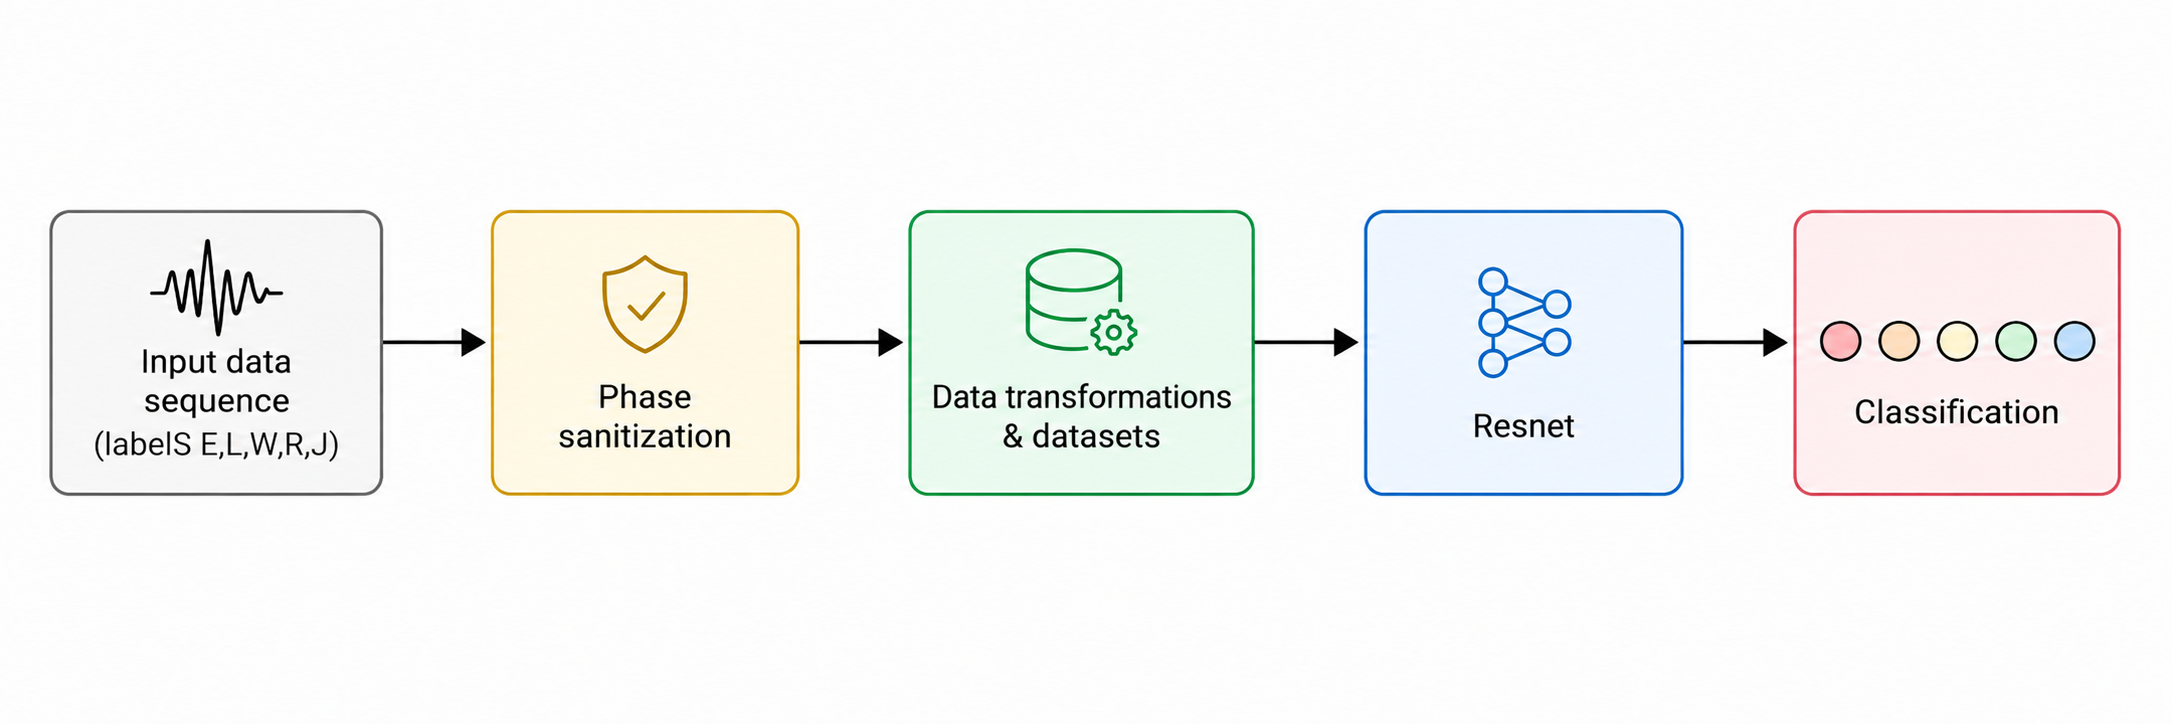
\includegraphics[width=1.0\linewidth]{processing_pipeline.png}
    \caption{Processing pipeline. The image was generated by AI.}
    \label{fig:processing_pipeline}
\end{figure}

In this section, we're going to explain the structure of the pipeline, designed for the analysis and processing of the input doppler traces; a sketch of the pipeline is depicted in the flow diagram in Figure \ref{fig:processing_pipeline}. In the following, all the processing steps:

\begin{enumerate}

    \item \textbf{Input data}: The raw Doppler traces, associated with specific activities (defined by the labels E, L, W, R, J), serve as the input. These traces are acquired using the techniques proposed by \cite{MeneghelloNN-2023} and \cite{MeneghelloDataset-2023}, as detailed in Section \ref{sec:model};
    
    \item \textbf{Phase sanitization and computing the Doppler Traces}: This step, using the techniques specified in Section \ref{sec:model}, filters environmental and hardware noise from the raw data to ensure its reliability for subsequent analysis. After that, the input data is computed and the data sequence is obtained, as described in Section \ref{sec:model};

    \item \textbf{Dataset transformation and creation}: Following the cleaning process, transformations are applied to the data to enhance the robustness of the model against variations in the input. The specific techniques applied in this step are detailed in Section \ref{sec:model};

    \item \textbf{Deep neural architecture and Classification}: The transformed data are processed by a Resnet (whose architecture is defined in Section \ref{sec:learning_framework}) to predict the most probable class associated with the input. The system then outputs a loss value (logits) based on the predict.
\end{enumerate}

% \textbf{On tailoring the paper structure to your needs:} The structure recommended for the previous sections is rather standard and could work for different papers with differing technical content, the structure and the paper content from here on highly depends on the type of paper, possibilities are: mostly based on theoretical analysis, showing experimental design/activity, proposing a new technique and analyzing its performance via experiments or simulation. For the HDA course we deal with machine learning and, in detail, with training and testing neural network architectures to perform some specific inference or classification task. The following structure and comments are specifically addressing this type of technical content.

% \textbf{Why having this section:} With this section, we start the technical description with a {\it high level} introduction of your work (e.g., processing pipeline). Here, you do not have to necessarily go into the technical details of every block/algorithm of your design, this will be done later as the paper develops. What I would like to see here is a high level description of the approach, i.e., which processing blocks you used, what they do (in words) and how these were combined, etc. This section should introduce the reader to your design, explain the different parts/blocks, how they interact and why. You should not delve into technical details for each block, but you should rather explain the big picture. \rev{Besides a well written explanation, I often use a nice diagram containing the various blocks and detailing their interrelations.}

% \noindent \textbf{Writing tips:} Sections, Figures and Tables are usually shortened as Sec., Fig., Tab. 
% \begin{itemize}
% \item \textbf{Cross referencing:} In Latex, cross referencing is easy. You need to label an object through the \texttt{\textbackslash label\{labelid\}} command and referencing it where you need it through the \texttt{\textbackslash ref\{labelid\}} command. 
% \item \textbf{Suggestion:} I suggest to cross reference a table using \texttt{Tab.\mytexttilde\textbackslash ref\{tab:tableid\}}, the same holds for figures and sections, by just replacing ``\texttt{Tab.}'' with ``\texttt{Fig.}'' and ``\texttt{Sec.}''. Of course when defining the table, you need to add a Latex command \texttt{\textbackslash label\{tab:tableid\}} in the right place inside the table Latex environment to \mbox{cross-link} it. The tag \texttt{tab:tableid} is user defined and is the identifier that you associate with the table in question. You could call it \texttt{pippo} of you wish, but I recommend to use something like ``\texttt{tab:tableid}'' for tables, ``\texttt{eq:eqid}'' for equations, ``\texttt{sec:secid}'' for sections and so forth, where \texttt{tableid} has to be unique for each table in the document. The same applies to figures and all other objects. I guess you got the idea. This will lead to a neat Latex code and will facilitate cross referencing while avoiding duplicate labels, especially in large Latex documents (think of a book for example). 
% \item \textbf{But what about the tilde?} When you write \texttt{Tab.\mytexttilde\textbackslash ref\{tab:tableid\}} Latex knows that \texttt{Tab.} and the corresponding table number \texttt{\textbackslash ref\{tab:tableid\}} must be displayed within the same line, i.e., they can never be broken across lines. This is nice and desirable I believe. I always use it for all referenced material, including citations; example: ``As done in\texttt{\mytexttilde\textbackslash cite\{suppa-wu-2019\}}.''
% \item \textbf{More about breaking stuff across lines} often times you have composed words, in line equations, etc. and for some reason you would like Latex to never break them across lines. Example: the Latex command \texttt{\textbackslash mbox\{Neural Networks (NN)\}} is processed by Latex so that ``\mbox{Neural Networks (NN)}'' is never broken across lines. I use this very often, also for inline equations that I do not want Latex to split across subsequent lines.
% \end{itemize}

\section{Signals and Features}
\label{sec:model}

\begin{figure}[h!]
    \centering
    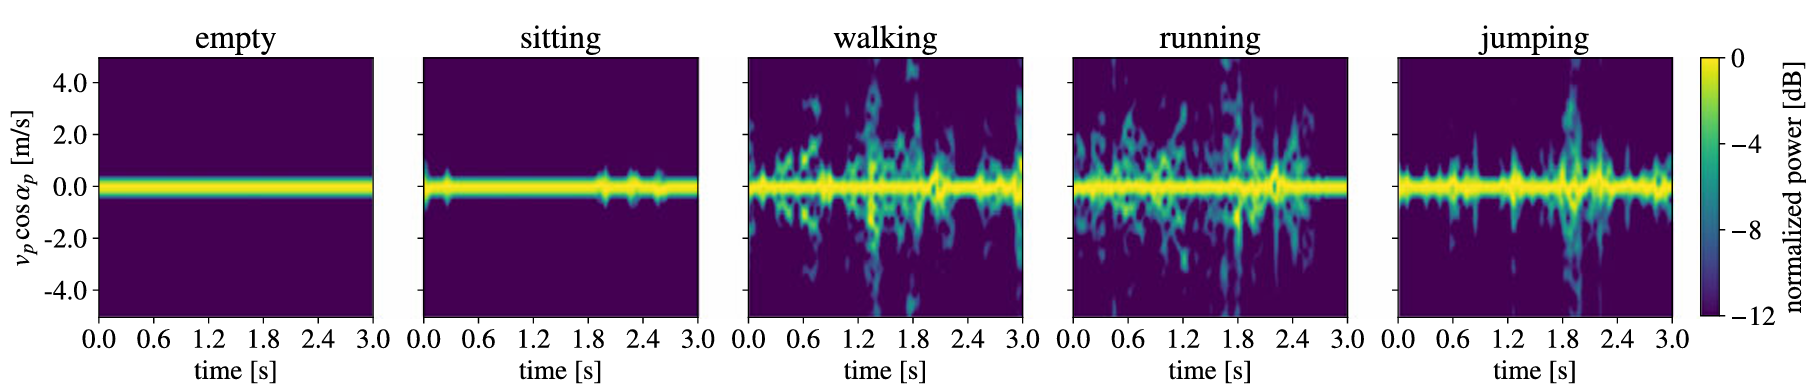
\includegraphics[width=1.0\linewidth]{labels.png}
    \caption{Spectograms of the five different activities and their associated labels, as proposed by \cite{MeneghelloNN-2023}}
    \label{fig:labels}
\end{figure}

As described by \cite{MeneghelloDataset-2023} and \cite{MeneghelloNN-2023}, the dataset comprises Wi-Fi Channel Frequency Response (CFR) data collected within an IEEE 802.11ac network. The signals were captured by a monitor node (an ASUS RT-AC86U router) while two terminals exchanged traffic on channel 42 operating at a center frequency of 5.21 GHz with an 80 MHz bandwidth while a human subject acted as a physical obstacle to the transmission by performing various activities. Due to constraints in computational resources, this experiment utilizes a subset of the labeled activities and subjects. Specifically, the evaluated activities are empty 'E', sitting 'L', walking 'W', running 'R', and jumping 'J' (Figure \ref{fig:labels}). Regarding the dataset split, the data from four subjects are allocated to the training and validation phases, while the data from a single, separate subject are reserved exclusively for testing.

About the computation of CFR, in \cite{MeneghelloNN-2023},the authors mathematically formulate the raw CFR acquired from commercial Wi-Fi devices communicating via Orthogonal Frequency Division Multiplexing (OFDM). The multi-path CFR across sub-channels is defined as:

\[ H_{k}(n) = A_{k}(n)e^{j\phi_{k}(n)} = \sum_{p=0}^{P-1} A_{p}(n)e^{-j2\pi(f_{c}+k/T)\tau_{p}(n)}\]

where $H_{k}(n)$ is the sub-channel response, $A_{k}(n)$ is attenuation, $\phi_{k}(n)$ is phase shift, $P$ is the path count, $A_{p}(n)$ is path attenuation, $f_{c}$ is carrier frequency, $T$ is OFDM symbol time, and $\tau_{p}(n)$ is path delay. This raw signal model contains non-ideal hardware phase artifacts that distort real-world measurements.\\

After that, there's a \textit{Sanitization phase}, in which this raw CFR is processesed by removing the phase offset, outputting a cleaned signal $\hat{H}_k$, which is computed as:

\[ \hat{H}_{k} \approx A_{p^*}e^{-j2\pi(f_{c}+k/T)\tau_{p^*}} H_{k}\]

where $\hat{H}_{k}$ is the corrected CFR for sub-channel $k$,  $A_{p^*}$ and $\tau_{p^*}$, are the amplitude and delay of the strongest reference path $p^*$, while  $H_{k}$ represents the isolated dynamic multi-path component required for detecting human activity.

Finally the last step of the preprocessing phase is the \textit{Doppler Trace Computation}, in which the sanitized CFR ($\hat{H}_k$) previously computed are transformed into Doppler spectrograms to isolate human movement velocity from static reflections. By arranging sanitized phase data into time-sequenced observation matrices and applying a short-time Fourier transform (STFT), temporal variations are converted into a Doppler spectrogram.
The physical movement model is defined as:

\[ v_{p}\cos(\alpha_{p}) = \frac{uc}{f_{c}T_{c}N_{D}}\]

where $v_{p}\cos(\alpha_{p})$ is the directional velocity of scatterer $p$,  $u$ is the discrete Doppler bin index associated with physical motion, $c$ is the speed of light,  $f_{c}$ is the central carrier frequency, $T_{c}$ is the sampling period between packets and $N_{D}$ is the Number of zero-padded signal samples. Specifically, the computation of Doppler traces is performed with the following parameters:

\begin{itemize}
    \item Number of channels estimates for Doppler computation per sample: 31
    \item Number of packets for sliding operations: 1
    \item Number of Doppler vectors per window: 340
    \item Number of samples for window sliding: 30
    \item Number of monitoring antenna: 4
\end{itemize}

Once the sanitized data are obtained, the following transformations are applied sequentially to the training dataset, in order to improve model generalization:

\begin{enumerate}
    \item \textbf{Gaussian noise}: Zero-mean additive white Gaussian noise ($\mu = 0$, $\sqrt{\sigma^{2}} = 0.05$) is injected into the data sequence to simulate signal fluctuations.
    \item \textbf{Uniform scale variation}: A scaling factor chosen uniformly from $[0.9, 1.1]$ is applied to randomly alter the apparent duration of the sequence.
    \item \textbf{Block masking}: A contiguous block representing $5\%$ of the total sequence length is randomly masked to train the model to handle missing data.
\end{enumerate}

To ensure unbiased evaluation, these transformations are disabled during the validation and testing phases. Specifically, the Gaussian noise and block masking parameters are set to $0$, and the scale variation factor is set to $1.0$. These transformations are applied dynamically upon dataset instantiation.

% Being a machine learning paper, I would have here a section describing the signals you have been working on. If possible, you should describe, in order, 
% \begin{enumerate}
% \item the measurement setup (if relevant), how input data is formatted (e.g., vectors of fixed size measured at regular sampling times), 
% \item how the signals were \mbox{pre-processed}, e.g., to remove noise, artifacts, fill gaps (missing points) or to re-interpolate the signals to represent them through a constant sampling rate, etc.
% \item after this, you should describe how {\it feature vectors} were obtained from the \mbox{pre-processed} signals. If signals are {\it time series} this also implies stating the segmentation / windowing strategy that you adopted, to then describe how you obtained a feature vector for each time window. Also, if you use existing feature extraction approaches, you may want to briefly describe them as well, in addition to (and before) your own (possibly new) feature extraction method.
% \end{enumerate}

% \rev{Last but not least, this section should also contain information on how you have split the dataset into training, validation and test sets. This will be briefly recalled within the ``Results'' section.}

\section{Learning Framework}
\label{sec:learning_framework}

In this section there are detailed descriptions of each block of the Resnet architecture adopted for the project.

% \subsection{Transformer-Encoder}

% \begin{figure}[H]
%     \centering
%     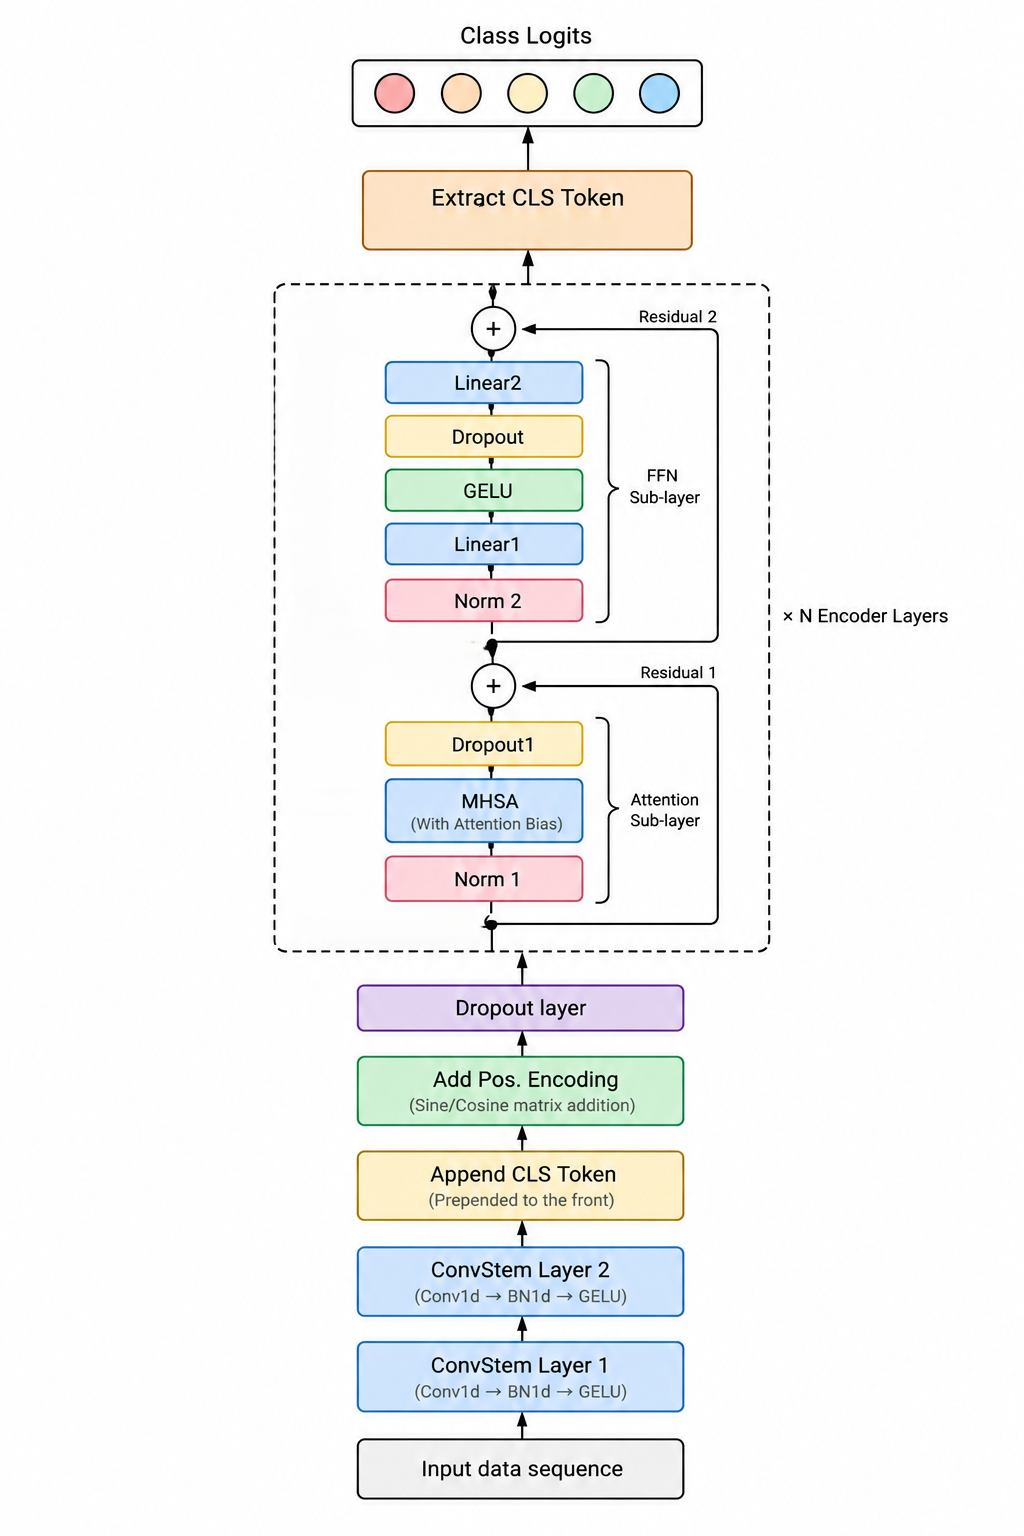
\includegraphics[width=0.45\linewidth]{encoder_architecture.png}
%     \caption{Transformer-Encoder architecture. The image was generated by AI.}
%     \label{fig:encoder_architecture}
% \end{figure}

% As depicted in Figure \ref{fig:encoder_architecture}, the input sequence is initially processed by a Convolutional STEM layer to capture local patterns and downsample the sequence length by a factor of four, easing the $O(n^2)$ computational complexity of subsequent attention steps. This STEM structure consists of two 1D convolutional layers with batch normalization and Gaussian Error Linear Unit ($\text{GELU}$) activations \cite{Hendricks-2016}:

% $$\text{Gelu}(x) = x \cdot \frac{1}{2} \left[1 + \text{erf}\left(\frac{x}{\sqrt{2}}\right)\right]$$

% where $\text{erf}(x) = \frac{2}{\sqrt{\pi}} \int_{0}^{x}{\exp(-t^2)dt}$. The first convolution accepts $\bm{x} \in \mathbb{R}^{F \times M}$ using parameters $K = 5, P = 2, S = 2$. The second layer operates on $\bm{\tilde{x}} \in \mathbb{R}^{M \times M}$ with parameters $K = 3, P = 1, S = 2$. After the second $\text{GELU}$ activation, a learnable \textbf{[CLS]} token is concatenated to aggregate global information for classification \cite{MeneghelloDataset-2023, MeneghelloNN-2023}. Next, positional temporal information \cite{Vaswani-2023} is injected using an alternating matrix $\bm{X}$ of size $J \times M$:

% $$\bm{X}_{(k, 2i)} = \sin\left(\frac{k}{10000^{\frac{2i}{M}}}\right), \quad \bm{X}_{(k, 2i+1)} = \cos\left(\frac{k}{10000^{\frac{2i}{M}}}\right)$$

% where $k$ is the token position index ($k = 0, \dots, J-1$) and $i$ is the dimension index ($i = 0, \dots, \frac{M}{2} - 1$). The enriched tensor passes through six identical encoder layers. Each layer executes Layer Normalization followed by self-attention computation \cite{Vaswani-2023}:

% $$\bm{A} = \text{softmax}\left(\frac{\bm{Q}\bm{K}^{T}}{\sqrt{d_k}} + \bm{bias}\right) \bm{V}$$

% where $\bm{Q} = \bm{x_{q}} \bm{W^{Q}}$, $\bm{K} = \bm{x_{k}} \bm{W^{K}}$, and $\bm{V} = \bm{x_{v}} \bm{W^{V}}$. After adding a residual connection and re-normalizing, the tensor enters a feed-forward network comprising a linear layer with $\text{GELU}$ activation, dropout, and a final linear projection. Ultimately, the representation of the \textbf{[CLS]} token is extracted from the final layer and passed to the classification head, where a Cross-entropy function

% is applied, in order to extract the logits.

The architecture of the resnet is developed in the following way:

\begin{enumerate}
\item \textbf{Input Preprocessing and Channel Injection Block:} The raw input batch tensor $x \in \mathbb{R}^{B \times H \times W}$ (where $B$ denotes batch size, $H$ represents time sequences, and $W$ represents feature dimensions) enters the forward pass and undergoes spatial reshaping via \texttt{x.unsqueeze(1)}. This transforms the tensor into a single-channel 2D representation $x \in \mathbb{R}^{B \times 1 \times H \times W}$, enabling 2D spatial convolution operators to ingest Doppler spectrograms directly;\\

\item \textbf{Convolutional Stem Block:} The single-channel tensor $x$ passes sequentially through \texttt{self.conv1}, \texttt{self.bn1}, \texttt{self.relu}, and \texttt{self.maxpool}:
\begin{itemize}
    \item \texttt{self.conv1} ($7 \times 7$ kernel, stride $s=2$, padding $p=3$): Downsamples spatial dimensions while projecting 1 input channel to $C_{\text{base}}$ channels (\texttt{base\_channels}):
    \begin{equation}
        x_{\text{conv1}} = \mathbf{W}_{\text{stem}} * x
    \end{equation}
    \item \texttt{self.bn1}: Standardizes activations per channel across the mini-batch to reduce internal covariate shift:
    \begin{equation}
        \hat{x} = \frac{x_{\text{conv1}} - \mu_B}{\sqrt{\sigma_B^2 + \epsilon}}, \quad y_{\text{bn1}} = \gamma \hat{x} + \beta
    \end{equation}
    
    \item \texttt{self.relu}: Applies element-wise rectification $\text{ReLU}(y) = \max(0, y)$;\\
    
    \item \texttt{self.maxpool} ($3 \times 3$ pool, stride $s=2$): Reduces spatial dimensions by half, yielding a feature map of shape $\left(B, C_{\text{base}}, \lfloor\frac{H}{4}\rfloor, \lfloor\frac{W}{4}\rfloor\right)$.\\
    
\end{itemize}

\begin{figure}[H]
    \centering
    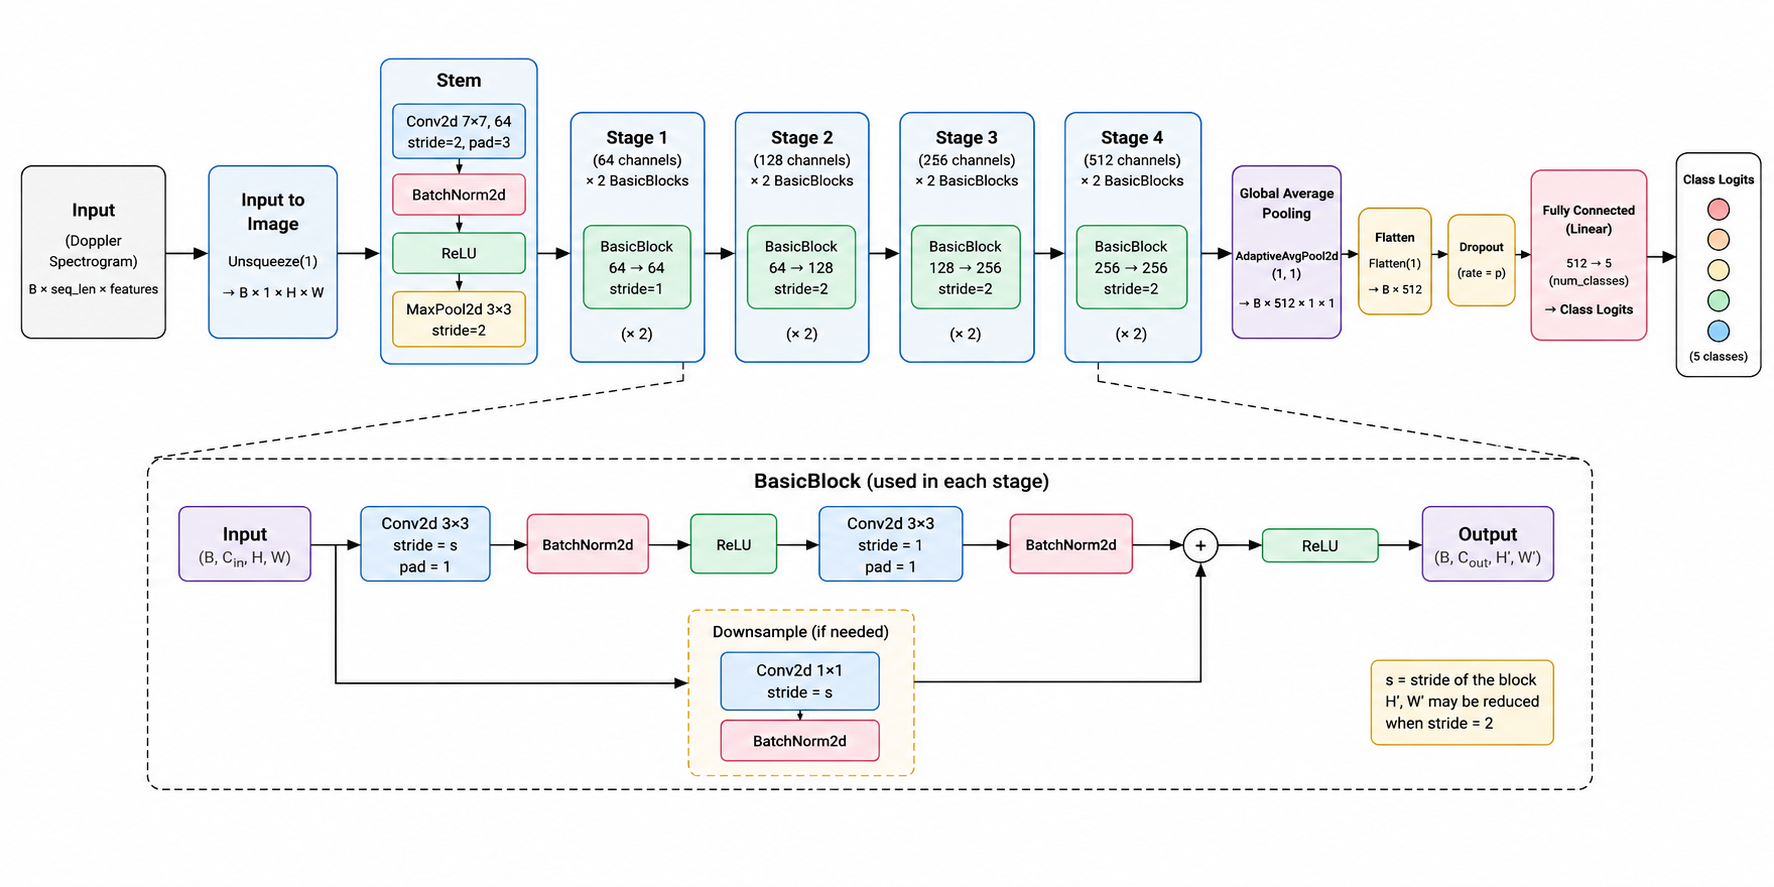
\includegraphics[width=1.0\linewidth]{resnet_architecture.png}
    \caption{Resnet architecture: image generated by AI}
    \label{fig:resnet_architecture}
\end{figure}

\item \textbf{Residual Deep Feature Extraction Stages (\texttt{BasicBlock} and \texttt{self.res\_layers}):}The tensor flows through sequential residual stages where spatial dimensions shrink by factor $2$ while channel depth doubles ($C_{\text{out}} = C_{\text{in}} \cdot 2$). Within each \texttt{BasicBlock}:
\begin{itemize}
    \item \textbf{Residual Branch Processing:} Input $x_{\text{block}}$ passes through two $3 \times 3$ convolutions with intermediate batch normalization and ReLU activation:
    \begin{equation}
        F(x_{\text{block}}) = \text{BN}_2\Big(\mathbf{W}_2 * \text{ReLU}\big(\text{BN}_1(\mathbf{W}_1 * x_{\text{block}})\big)\Big)
    \end{equation}
    
    \item \textbf{Shortcut Projection (\texttt{self.downsample}):} The input is saved as $h(x_{\text{block}}) = x_{\text{block}}$. If stride $s \neq 1$ or $C_{\text{in}} \neq C_{\text{out}}$, \texttt{self.downsample} adjusts dimensions via $1 \times 1$ convolution: $h(x_{\text{block}}) = \text{BN}_{\text{ds}}(\mathbf{W}_{\text{ds}} * x_{\text{block}})$;\\
    
    \item \textbf{Residual Addition and Regularization:} The shortcut is added element-wise before non-linear activation:
    \begin{equation}
        y_{\text{block}} = \text{ReLU}\big(F(x_{\text{block}}) + h(x_{\text{block}})\big)
    \end{equation}
    Stochastic feature dropout (\texttt{self.dropout}) zeroes activations with probability $p = \text{\texttt{dropout\_rate}}$ to prevent co-adaptation;\\
\end{itemize}

\item \textbf{Global Temporal Aggregation and Linear Head:} Spatial dimensions of feature maps $x \in \mathbb{R}^{B \times 8C_{\text{base}} \times H' \times W'}$ are collapsed into a scalar per channel by Adaptive Average Pooling (\texttt{self.avgpool}):
\begin{equation}
    x_{\text{pool}}(c) = \frac{1}{H' \times W'} \sum_{i=1}^{H'} \sum_{j=1}^{W'} x(c, i, j)
\end{equation}
The resulting tensor, as final step, is flattened via \texttt{torch.flatten(x, 1)} into $x_{\text{flat}} \in \mathbb{R}^{B \times 8C_{\text{base}}}$, subjected to dropout, and projected to category logits $z \in \mathbb{R}^{B \times N_{\text{classes}}}$ via \texttt{self.fc} ($\mathbf{W}_{\text{fc}} x_{\text{flat}} + b_{\text{fc}}$);\\

\item \textbf{Weight Initialization}: Initial weights of convolutional and linear layers are initialized using Xavier uniform initialization to bound layer output variances:
\begin{equation}
    W \sim U\left(-\sqrt{\frac{6}{n_{\text{in}} + n_{\text{out}}}}, \sqrt{\frac{6}{n_{\text{in}} + n_{\text{out}}}}\right)
\end{equation}

\end{enumerate}
% Here you finally describe the learning strategy / algorithm that you conceived and used to solve the problem at stake. A good diagram to exemplify how learning is carried out is often very useful. In this section, you should describe the learning model, its parameters, any optimization over a given parameter set, etc. You can organize this section into \mbox{sub-sections}. You are free to choose the most appropriate structure.

% Note that the diagram that you put here differs from that of Section~\ref{sec:processing_architecture} as here you show the details of how your learning framework, or the core of it, is built. In Section~\ref{sec:processing_architecture} you instead provide a high-level description of the involved processing blocks, i.e., you describe the {\it processing flow} and the rationale behind it.

% \noindent \textbf{On math typesetting:} there are many Latex tricks that you should use to produce a high quality technical essay. A few are listed below, in random order:
% \begin{itemize}
% \item \textbf{Vectors and matrices:} $x$ is a scalar, whereas $\bm{x}$ (in bold) is a vector, and $\bm{X}$ is a matrix with elements $\bm{X} = [x_{ij}]$. For bold symbols you may use the \texttt{\textbackslash bm} Latex command, e.g., \texttt{\textbackslash bm(x)}.
% \item \textbf{Operators:} such as $\max$, $\min$, $\arg\!\max$, $\arg\!\min$ and special functions such as $\log(\cdot)$, $\exp(\cdot)$, $\sin(\cdot)$, $\cos(\cdot)$ are obtained through specific latex commands \texttt{\textbackslash min}, \texttt{\textbackslash max}, \texttt{\textbackslash arg\textbackslash!min}, \texttt{\textbackslash arg\textbackslash!max}, \texttt{\textbackslash log}, \texttt{\textbackslash exp}, \texttt{\textbackslash sin}, \texttt{\textbackslash cos}, etc. Use them! $log$, $exp$, $min$, $sin$, $cos$, etc., look ugly.
% \item \textbf{Sets} can be represented through calligraphic fonts, e.g., $\mathcal{S}$, $\mathcal{F}$, $\mathcal{B}$, etc., obtained using the Latex command \texttt{\textbackslash mathcal{\{S\}}}, etc.
% \item \textbf{Equations:} for a single equation use the \texttt{equation} Latex environment. Example: 
% \begin{equation}
% \label{eq:sigmoid}
% \sigma(x) = \frac{1}{1+e^{-x}}.
% \end{equation} 
% Now, using round brackets $($ and $)$ we get
% \begin{equation}
% \label{eq:sigmoid_comma}
% \sigma(x) = (\frac{1}{1+e^{-x}}),
% \end{equation} 
% but this looks ugly, you should use ``\texttt{\textbackslash left (}'' for ``$($'' and ``\texttt{\textbackslash right )}'' for ``$)$'', obtaining
% \begin{equation}
% \sigma(x) = \left ( \frac{1}{1+e^{-x}} \right ).
% \end{equation} 
% \item \textbf{Punctuation:} Displayed equations are usually considered to be part of the text and, in turn, they will get the very same punctuation as if they were inline with the text (and part of the sentence). If the sentence ends with a displayed equation, the equation gets a period ``.'' right after it, see Eq.~(\ref{eq:sigmoid}). iI the equation is instead part of a running sentence, which is continued after it, then the equation may be ended by a ``,'' as in Eq.~(\ref{eq:sigmoid_comma}). Use the standard grammar rules and your good sense of flow to assess how equations should be punctuated, I usually read through as if they were plain text.
% \end{itemize} 

